\documentclass[12pt,a4paper]{scrartcl}
\usepackage[utf8]{inputenc}
\usepackage{amsmath}
\usepackage{amsfonts}
\usepackage{amssymb}
\usepackage{hyperref}
\usepackage{graphicx}
\author{Matthias Larisch\\\url{github@matthias-larisch.de}\\\url{https://github.com/NerdyProjects/}}
\title{IEEE 802.1x authentication password exposure in WPA-Enterprise networks}
\begin{document}
\maketitle
802.1x authentication is widely deployed in wired and wireless networks. While theoretically most of the techniques described here should apply to all kinds of IEEE 802.1x authentication, this paper focuses on wireless networks using the WPA Enterprise or WPA2-Enterprise (IEEE 802.11i with IEEE 802.1x authentication).
The required network structure is given in fig. \ref{f:wpa-eap-structure} and consists of an access point device which additionally features the role of an authenticator, an authentication server and the wireless node (supplicant).
To access the network, the supplicant has to authenticate against the authentication server via EAP packets. Other network traffic will only be allowed after the authentication server accepts the supplied credentials.

\begin{figure}
  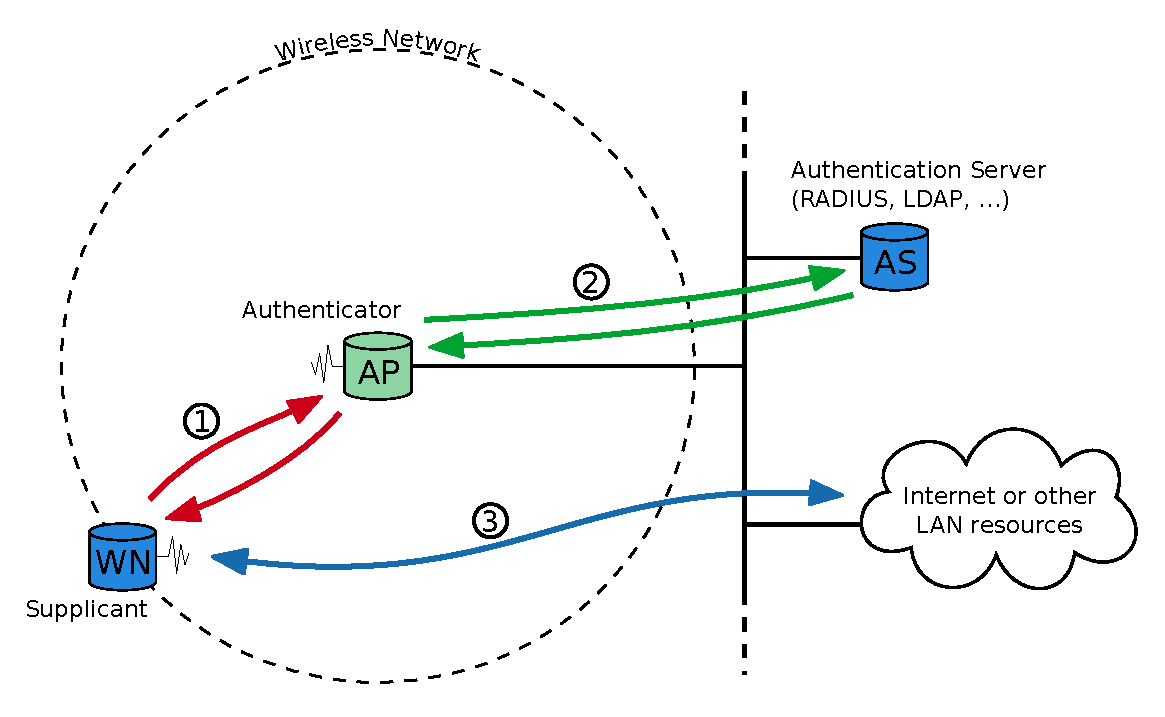
\includegraphics[width=\textwidth]{8021x}
  \caption{Roles for 802.1x authentication, Source: Wikipedia User Rohieb, Creative Commons}
  \label{f:wpa-eap-structure}
\end{figure}
There are lots of different authentication methods available, some using a PKI (public key infrastructure) for authenticating the supplicant to the authentication server and sometimes vice-versa, some use password authentication in different more or less secure ways.
The following weakness is analysed for the common deployed authentication method PEAP/MSCHAPv2, used for example in the well known eduroam network. However, the majority of facts should be applicable to all password authentication modes.
\section{802.1x authentication in detail}
Upon accessing the network, the supplicant is able to communicate to the authenticator via EAPOL packets. Those packets are then forwarded to the authentication server, commonly as RADIUS packets, but there is also integrated authenticator/authentication server software available (e.g. hostapd).
As at this early stage none of those packets are encrypted at the 802.11 MAC layer (using known WPA AES/RC4 methods), a secure authentication must be guaranteed by the authentication protocol itself.
Therefore, different EAP methods are defined.
In addition, some of these methods allow adding an additional layer, that is, transporting regular EAP packets as payload of an EAP packet.
In this way, unencrypted or otherwise known as unsafe authentication methods may be used on this inner layer, when the outer layer is reliably encrypted and authenticated.
All EAP methods use an identity to describe the user.
This identity can differ in outer and inner layer EAP method and therefore two phase methods allow transmitting an anonymized identity over the untrusted channel which may be used to determine the targeting authentication server (this is used in eduroam networks so inner layer authentication is always done at the home organisation of the connecting client even when roaming)

The following paragraphs describe some common authentication methods.

\paragraph{EAP-TLS} uses PKI with client and server certificates.
Both the client and the server are able to validate the certificate chain where the server can additionally match the common name or other attributes of the client certificate.
Getting EAP-TLS in the field is complicated as each client has to be supplied with a certificate.
As the PKI can directly ensures mutual trust, no further (password based) authentication is needed.


\paragraph{EAP-TTLS and EAP-PEAP} are similar to TLS except for a lack of a client certificate.
A secure TLS tunnel is established and allows another authentication method be used inside \cite{ttlspeap}.
While TTLS traditionally only supported the transmission of RADIUS-like attribute-value pairs, today TTLS and PEAP are implemented allowing all other EAP authentication methods inside the tunnel.
The authenticity of the authentication server (and therefore the whole tunnel) is optionally ensured by verifying the CA certificate.
Some supplicants also allow for additional certificate attributes to be checked (eg wpa\_supplicant directive subject\_match).
The german Wikipedia article on eduroam \cite{wiki-eduroam} describes security implications of certificate checking since 2008 but does not propose a way to apply those checkings as the author does not know of any GUI for supplicants that allow setting trustworthy certificate checking options, although some supplicants have the neccessary options implemented.

\paragraph{PAP (Password Authentication Protocol)} is a relict from the ancestors of EAP, PPP.
It uses clear text username and password authentication and is sometimes used as inner layer to EAP-TTLS.

\paragraph{GTC (Generic Token Card)} is a method applicable to token cards with challenge response authentication.
Common implementation uses GTC to supply cleartext passwords.
RFC3748 explicitly forbids the usage of EAP-GTC with cleartext passwords in the absence of a protected tunnel with server authentication. The author did not observe any supplicant obeying to this RFC. In addition, the supplicant may not be able to determine if the server is trustworthy (see CA reuse problems described later).

\paragraph{MS-CHAPv2} is a challenge/response based method firstly published by Microsoft.
It provides mutual authentication between client and server and does not expose passwords by using an MD4 hash of the user password.
MSCHAPv2 is considered broken at least since 2012, when David Hulton and Moxie Marlinspike published their results on getting the MD4 hash of the user password by cracking a single 56 bit DES key.
The MD4 hash is sufficient to authenticate as the targeted user or decrypt all traffic.
As two bytes of the MD4 hash can be trivially computed by breaking a 16 bit DES key, even very large precomputed password tables can be used extremely fast to match precomputed passwords against a given challenge and response.
There is also an internet service which offers completely covered MS-CHAPv2 cracking in 24 hours for \$100 per challenge/response.
To avoid misunderstandings this only leads to the NTLM-Hash of the user password which is sufficant for some further attacks but not all.
Dictionary and brute force attacks on NTLM hashes may be very fast when using rainbow tables therefore MSCHAPv2 cannot be considered a secure authentication at all and must never be used over an untrusted channel (so we get a little bit more obscurity than GTC would provide but as even the Wikipedia article states: "Enterprises who are depending on the mutual authentication properties of MS-CHAPv2 for connection to their WPA2 Radius servers should immediately start migrating to something else." (Moxie Marlinspike, \cite{wiki-wpa})

\paragraph{EAP-SIM and EAP-AKA} 
There are a lot more authentication methods available.
SIM and AKA methods are special purpose to mobile devices featuring a GSM/UMTS sim card.
The IMSI (international mobile subscriber identity) - an unique sim card identifier - or an anonymous identifier may be used together with other information including the network operator as a username.
Encryption keys are generated by generating challenges to the sim card, so the encryption basically relies on the security of the secret key stored inside the sim card ($K_i$).

Other methods include MD5, FAST and EKE.
Especially EKE may be interesting for further research as it allows a secure mutual authentication by a password without a need for an encrypted outer channel.
The corresponding RFC 6124 was published in 2011 so there should be very little end device support for EAP-EKE as for now.

\section{Attack scenarios}
Different scenarios must be taken into account to evaluate the vulnerabilities of a network.
Special setups may increase the vulnerability of a given system (e.g. by password reuse).

\subsection{Man in the middle}
A classical attack is the man in the middle (MITM).
The attacker places itself somewhere in the network to redirect the traffic intended for some other station to itself.
It may additionally communicate with the original destination station so the victims have no idea they are being attacked.
In 802.1x authentication, this attack is possible because missing or failing authentication of the server towards the client.
Even CA-based authentication chains may be broken, as will be discussed later in this paper.

A MITM attack during authentication may lead to one or two of the following:
\begin{itemize}
  \item Leading the target onto the attackers network for application protocol MITM attacks or
  \item stealing the login credentials of the user.
\end{itemize}

For both scenarios it is neccessary that the server's authenticity is not effectively ensured.
Because of the possible two-layer authentication in EAP networks, it might be possible for the inner layer to discover a rogue server.
Both EAP-TTLS and EAP-PEAP, the only outer layer protocols, may be secured by a CA certificate which may or may not be sufficient to prove the server's authenticity.
All cleartext password inner authentications are not able to authenticate the server, which would also be too late as the attacker already got the login credentials at this stage.
MSCHAPv2 implements the challenge and response in a way which ensures mutual authenticity of the server and the client so the client may detect a rogue server in the authentication response as the server has to know the NTLM hash of the users password to generate that.
Anyway, the attacker already got the challenge and the client's response at this time and may happily upload both to cloudcracker to receive the NTLM hash within a day \cite{cloudcracker}.

\subsection{Impersonation}
An attacker who succeeded in a MITM attack may use this information to impersonate the original user.
In wireless network environments, this goes one step further than on the internet as total privacy for the attacker is free as long as he also uses the original user's hardware address (commonly referred as MAC), which he also got during the MITM.
Wifi localisation may be outwitted for hours in a crowded place or by redirecting the traffic over a small, unsuspicious device (e.g. a smartphone) as the wifi operator should not be looking for the user before he gets any abuse reports which may be hours or even days after a possible incident.


\section{The complete fail of 802.1x authentication on WiFi networks}
The preceeding sections may already have given a clue to avoid using some authentication methods.
For simplicity, a lot of networks and especially the eduroam network targeted in this paper operate password authenticated EAP-TTLS-MSCHAPv2 or EAP-PEAP-MSCHAPv2 networks.
Although this might be acceptable in theory, it is unresponsible and totally unacceptable in practice.
Wireless clients, especially mobile devices, tend to allow other authentication methods to be used with stored credentials.
Therefore, an attacker may setup a network with SSID eduroam and WPA-Enterprise encryption using an EAP authentication server configured for EAP-PEAP-GTC with EAP-PEAP-MSCHAPv2 fallback.
A huge amount of clients will successfully initiate the TLS session and "securely" authenticate with their cleartext credentials to the attackers authentication server.
As the legal situation is unknown, so far only a biased private evaluation of this attack with consenting subjects has taken place.

While an enterprise network may detect such an attacker using its intrusion detection system, in case of eduroam there is no need to execute the attack physical near to an operating network.
Anyone may just observe the massive amount of probes for an eduroam network on a wednesday or saturday evening in every major city.
Every probe is a potential victim.

\subsection{What about CA security?}
Eduroam, as deployed at the University of Oldenburg at time of writing, uses a server certificate for its authentication server that is derived from the Deutsche Telekom Root CA 2.
Therefore, every client is (well... SHOULD BE) encouraged to set the CA certificate for eduroam to Deutsche Telekom Root CA 2.
So, everyone is safe here.\newline
Wait.\newline
Oh.\newline
Not.\newline
Every student can get a free certificate from the universities PKI which also is derived from the Deutsche Telekom Root CA 2. You just have to apply for it at \cite{ol-pki}.\newline
Uups.

By the way: Have you ever seen someone really configuring this complicated CA certificate?
It needs to be downloaded manually to the device.
Oh, then there would be not a bit of more work to use a DEDICATED CA only for the radius which would bring full mitigation of the described attack, as long as anybody is enforced to use this (but still most users won't...)

\subsection{The attacker got the password. Now, what?}
Most universities use the eduroam login for additional services.
This is critical as most of these services contain sensitive information:
\begin{itemize}
  \item Stud.IP
  \item Groupware: E-mail, calendar, contacts, tasks, notes
  \item Home-directory (including windows profile data, may be used for installing targeted, custom made virusses on workstation PCs)
  \item for some users additional adminstrative services such as websites, exam management, maybe access to critical (IT) infrastructure?
\end{itemize}

\subsection{Attack analysis}
We are encountering two/three main problems here:
\begin{enumerate}
  \item Missing server authentication
  \item Missing enforcement of authentication method
  \item Password reuse for multiple services
\end{enumerate}

It is crucial to understand that there are no countermeasures for the networkoperator against items one and two.
They purely depend on the end device settings and while you can enforce the user not giving her or his password to somebody else you cannot trust him making the right settings on his device.

\paragraph {Server authentication}
Eduroam's server authentication depends purely on the CA certificate which is broken in the way shown above.
Mitigations are possible by manual intervention in wpa\_supplicant's config:
\begin{verbatim}
'subject_match="/C=DE/ST=Niedersachsen/L=Oldenburg/O=Universitaet
   Oldenburg/OU=IT-Dienste/CN=radsrv.uni-oldenburg.de"'
'ca_cert="hash://server/sha256/c278ebaad3f851a39a3eeb991e5fb9999a
   cdaeb11ce50980548d7974913c5fb5"'
\end{verbatim}

This also leads to a simpler setup because one does not need to manually copy the custom CA certificate to the device.
Certificate checking by CN is safe as long as the CA chain is not compromised.

Apple devices seem to support setup profiles which may include additional server certificate checking as setup recommendations from other universities suppose.
%http://www.hs-esslingen.de/de/hochschule/service/rechenzentrum/mobile-net-wlan-openvpn/anleitungen-mobile-net/apple-mac-os-x-107lion-und-hoeher.html
The author has not seen any other device with stock support for server certificate validation further than (broken) CA certificate validation.

Additional research after starting this paper lead to an analysis from another university student, referenced in \cite{h4des}.
Interestingly, Stefan Winter, involved with eduroam europe R\&D, responded to the very interesting blog post and stated that a university with the given setup (and especially setup manuals) violated eduroams terms and services.

It is also made clear that mostly Android phones (with Android less than 4.3) suck at wifi security configuration and the eduroam provisioning tool will provide secure profiles for all Apple devices.
While I did not confirm that, those profiles sound like they do server certificate fingerprint checking which would be enough to ensure a server's authenticity and so may be considered secure.

No matter what validation methods are recommended here, the user may not be forced to set his device up in the right way.

Simply clicking on eduroam at the wireless networks list on most devices does not even ask for any further server validation.
This allows credential stealing as described by setting the authentication method to cleartext or easily crackable methods.


\paragraph{Client authentication method}
Eduroam administrators cannot enforce the client to use a specific authentication method on malicious authentication servers or access points.
This leads to a very concerning vulnerability as widely deployed clients were seen accepting unsecure authentication methods over an untrusted channel.
The author of this paper did not look deep enough into the situation to classify vulnerable devices.
Though, successful attacks of this kind (device accepts EAP-PEAP-GTC with cleartext password) have been executed against phones of all big vendors of mobile devices.
This seems to be the consequence of adding the scanned eduroam network where some Android phones create a profile without any preselected authentication method.
Setting the authentication method manually to EAP-PEAP-MSCHAPv2 fixes this issue for all examined devices.
As this setting has to be entered manually by the user, the network operator have no possibility to enforce it.
This issue does not seem to be common knowledge and leads (after the unauthenticated outer tunnel is established) to the biggest rate of exposed passwords.

\paragraph{MSCHAPv2 vulnerability}
While the reader is strongly encouraged to consider the original sources the following section gives a short overview over the MSCHAPv2 vulnerabilities which allows dictionary attacks to be executed very effectively.
MSCHAPv2 is a challenge response authentication method using random but known server and client challenges (so precomputation for whole challenge response cycles is not possible).
The \texttt{ChallengeHash} is derived from those known, random sources.
The weird algorithm splits it into three parts and encrypts each part with 7 bytes of the NTLM hash as DES key.
As the NTLM hash is only 16 bytes long, the last key part does only contain 2 bytes of the hash and is zero padded.
As this keyspace, containing $2^{16}$ possible keys, is very small, two bytes of the NTLM hash can be computed in about one second on every modern system.
Those two bytes can directly be used as an index into a precomputed Password $\rightarrow$ NTLM hash table so only about $\frac{1}{65536}$ of it has to be tested.
If the dictionary attack fails due to a too small dictionary, the rest of the NTLM hash can be gathered in less than $2^{56}$ DES encryptions.
Specialised hardware could do this in less than 24 hours some years ago, even better hardware could be built these days (the author is not aware of any attempts so far).
A single ATI Radeon HD7850 GPU (about \$150) needs about 500 days testing the entire 56 bit DES keyspace \cite{des-gpu}.
Affordable (less than \$20k) FPGA implementations should also be possible.
The online service cloud cracker offers cracking a MSCHAPv2 challenge response to a NTLM hash in 24 hours for just \$100.
When the NTLM hash is known, regular MD4 rainbow tables could be used to generate the original password in less than an hour.

The reader should be encouraged not to trust MSCHAPv2.

In conclusion, the security of the eduroam user password depends entirely on the verification of the authentication servers CA certificate which is only done by a very small amount of clients.
Therefore, the eduroam password can not be considered private and any data accessible by it should be considered public.

\subsection{Countermeasures}
\begin{enumerate}
  \item The author strongly recommends \textbf{using a single dedicated password for the unsecure eduroam authentication}. In addition, other services should be tested for their authentication vulnerabilities.
  \item A private CA should be used only for eduroam so authenticity of the authentication server can be assured just by validating the CA certificate. Still, the user has to set up this right to be effective!
  \item All users should be notified of the effects a wrong wifi profile setting may have. Ideally, a brief and easily understandable version of this paper should be published with the eduroam setup instructions.
  \item Preset profiles with secure settings should be published for devices that support them (eg Apple devices; see eduroam CAT)
  \item \textbf{The eduroam password should always be considered public as long as it can be used for any insecure authentication method as described in this paper and must therefore not be used for any services requiring specific user permissions}
\end{enumerate}

\subsection{Conclusion}
Although it is clear now that the main issue described in this paper is considered by the eduroam organisation and secure ways for network access are propesed by the organisation, the analysis shows that those methods are not wildly deployed.
In some cases (e.g. Android devices before 4.3, which are clearly the most deployed wireless clients) there is no possibility for a secure authentication given the proposed methods.
That is why all users should be informed about the existing issues and an alternate authentication method should be provided.

The very least thing a responsible network administrator should to is to provide sufficient configuration manuals.
This is - at least for the University of Oldenburg at time of writing - not the case.
Even more than three months after disclosing an earlier version of this paper to the responsible administrators.

See my github account \cite{gh-nerdy} for neccessary hostapd patches for a testsetup which may be used to get login credentials of very wrong configured end devices (e.g. no CA validation, no force of MSCHAPv2 - even with CA validation if you got a Deutsche Telekom CA 2 derived certificate).
You may get the MSCHAPv2 credentials as well, if the device is at least in parts correctly configured.

There are also patches against Cyanogenmod 11 so you may compile a hostapd for your Android phone and collect a nice amount of login credentials your whole day long.

Disclaimer: This may be illegal in some countries. As you are technically doing no harm to any network and don't sniff anything (the devices send the passwords \textbf{to you}) this could possibly also be legal here in Germany. 

An additional patch for airdump-ng patches airodump in a way to automatically deauthenticate strong clients from any other accesspoint (except your rogue one) and may be nice for a walk over your campus to collect hundreds of login attempts.
This clearly is illegal as you inject packages into a wireless connection you did not initiate.

\begin{thebibliography}{9}

\bibitem{ttlspeap}
  \url{www.opus1.com/www/whitepapers/ttlsandpeap.pdf}

\bibitem{cloudcracker}
  \url{https://www.cloudcracker.com/blog/2012/07/29/cracking-ms-chap-v2/}

\bibitem{des-gpu}
  \url{http://www.reddit.com/r/crypto/comments/162ufx/research\_project\_opencl\_bitslice\_des\_bruteforce/}
\bibitem{wiki-eduroam}
  \url{http://de.wikipedia.org/wiki/Eduroam#Sicherheitsbedenken}
\bibitem{wiki-wpa}
  \url{http://en.wikipedia.org/wiki/Wi-Fi_Protected_Access#MS-CHAPv2}
\bibitem{ol-pki}
  \url{http://www.pki.uni-oldenburg.de/}
\bibitem{h4des}
  \url{http://h4des.org/blog/index.php?/archives/341-eduroam-WiFi-security-audit-or-why-it-is-broken-by-design.html}
\bibitem{gh-nerdy}
  \url{https://github.com/NerdyProjects/hostapd-wpe-extended}
\end{thebibliography}
\end{document}
